\documentclass{article}

\usepackage{alltt}
\usepackage{amsmath}
\usepackage{amssymb}
\usepackage{amsthm}
\usepackage{bm}
\usepackage{changepage}
\usepackage{color}
\usepackage{fancyhdr}
\usepackage{float}
\usepackage[T1]{fontenc}
\usepackage{graphicx}
\usepackage[margin=0.8in]{geometry}
\usepackage{listings}

\pagestyle{fancy}

\lhead{Ryan Gibson}
\rhead{$k$-means using Nvidia accelerator(s)} 

\setlength\parindent{0pt}

\newcommand{\CPP}{C\nolinebreak[4]\hspace{-.05em}\raisebox{.22ex}{\footnotesize\bf ++}}
\DeclareFixedFont{\ttb}{T1}{txtt}{bx}{n}{12} % for bold
\DeclareFixedFont{\ttm}{T1}{txtt}{m}{n}{12}  % for normal

% Custom colors
\definecolor{deepblue}{rgb}{0,0,0.5}
\definecolor{deepred}{rgb}{0.6,0,0}
\definecolor{deepgreen}{rgb}{0,0.5,0}
\definecolor{dkgreen}{rgb}{0,0.6,0}

\begin{document}	
	The parallel algorithm (source code provided on the following pages) differs from the obvious sequential solution in a few key ways:
	\begin{itemize}
		\item ``Closest centroid'' cluster assignments are computed one point per thread.
		\item A sum reduction is used to combine the per-thread computations into per-block values.
		\item Two more block sum reductions are performed to reduce the values into a single block for the purposes of updating centroid positions.
		\item Branch prediction optimizations were removed since the CUDA architecture does not benefit from branches being taken more or less frequently.
	\end{itemize}

	Let $C = \frac{k \cdot n \cdot h}{t}$ be the computation rate where $1 \leq k \leq 1000$ is the number of clusters (means), $1 \leq n \leq 10^8$ is the number of points (in 2D), $h$ is the number of iterations until convergence, and $t$ is elapsed time (in seconds). Then, on a system with an E5-2650v3 CPU and TITAN V GPU,
	\begin{itemize}
		\item Our sequential code's performance peaked at ${\sim} 950$ million computations per second (across all parameter choices in these ranges).
		\item Our parallel code's performance peaked at ${\sim} 65$ billion computations per second (across all parameter choices in these ranges).
	\end{itemize}
	This constitutes approximately a 70x speedup (keeping in mind that a single core of the E5-2650v3 CPU and the entirety of a TITAN V are drastically different architectures).\\
	
	You can gain a significant speedup when $k$ is large by just using atomic CUDA operations (e.g. we've observed up to ${\sim}575$ billion computations per second for $k=1000$), but in practice $k$ is usually small, so we've intentionally avoided this solution.
	
	\begin{figure}[H]
		\begin{center}
			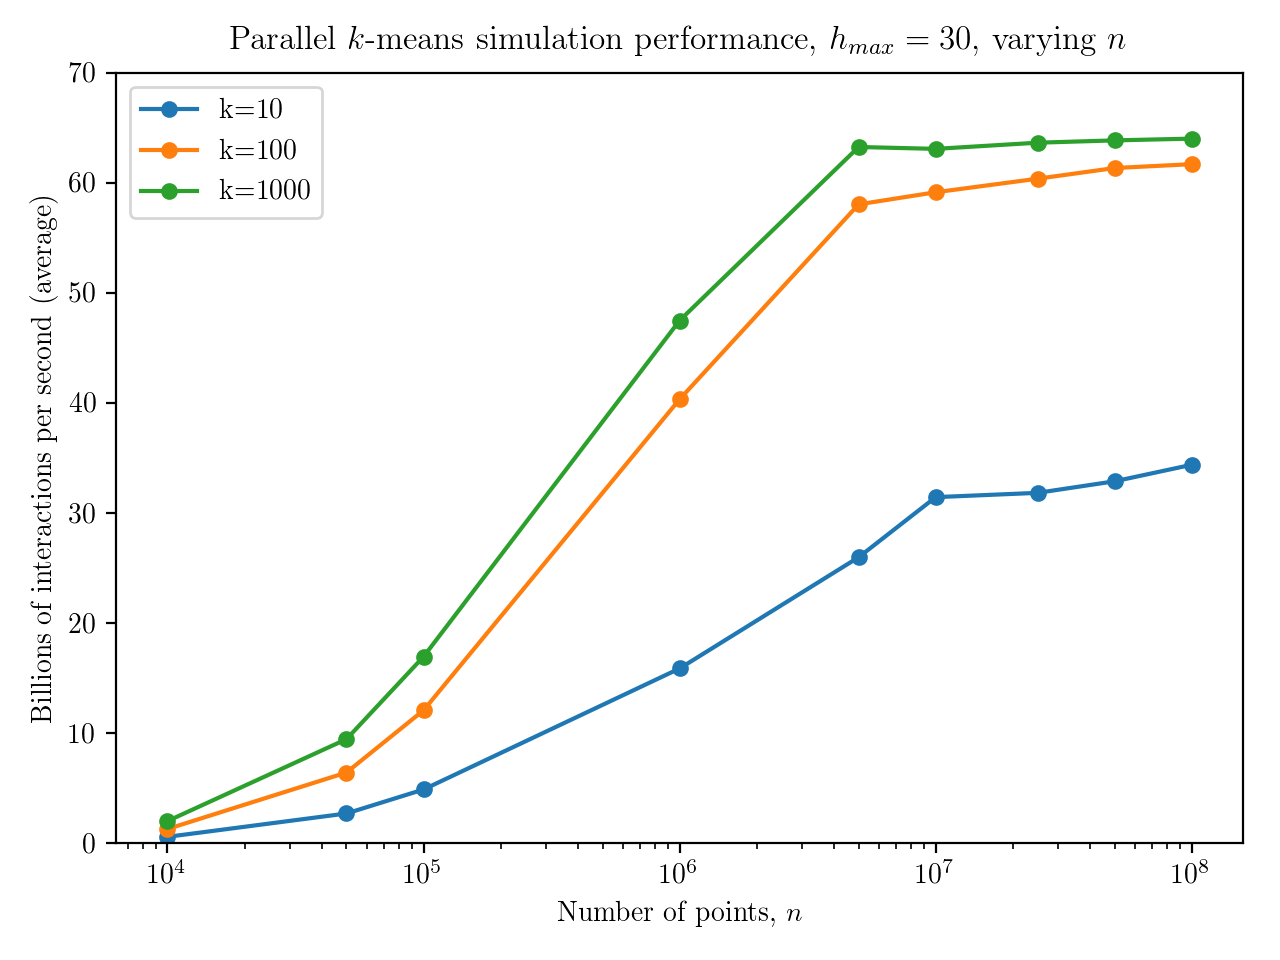
\includegraphics[width=5.2cm]{figures/perf_plot1_log.png}\quad
			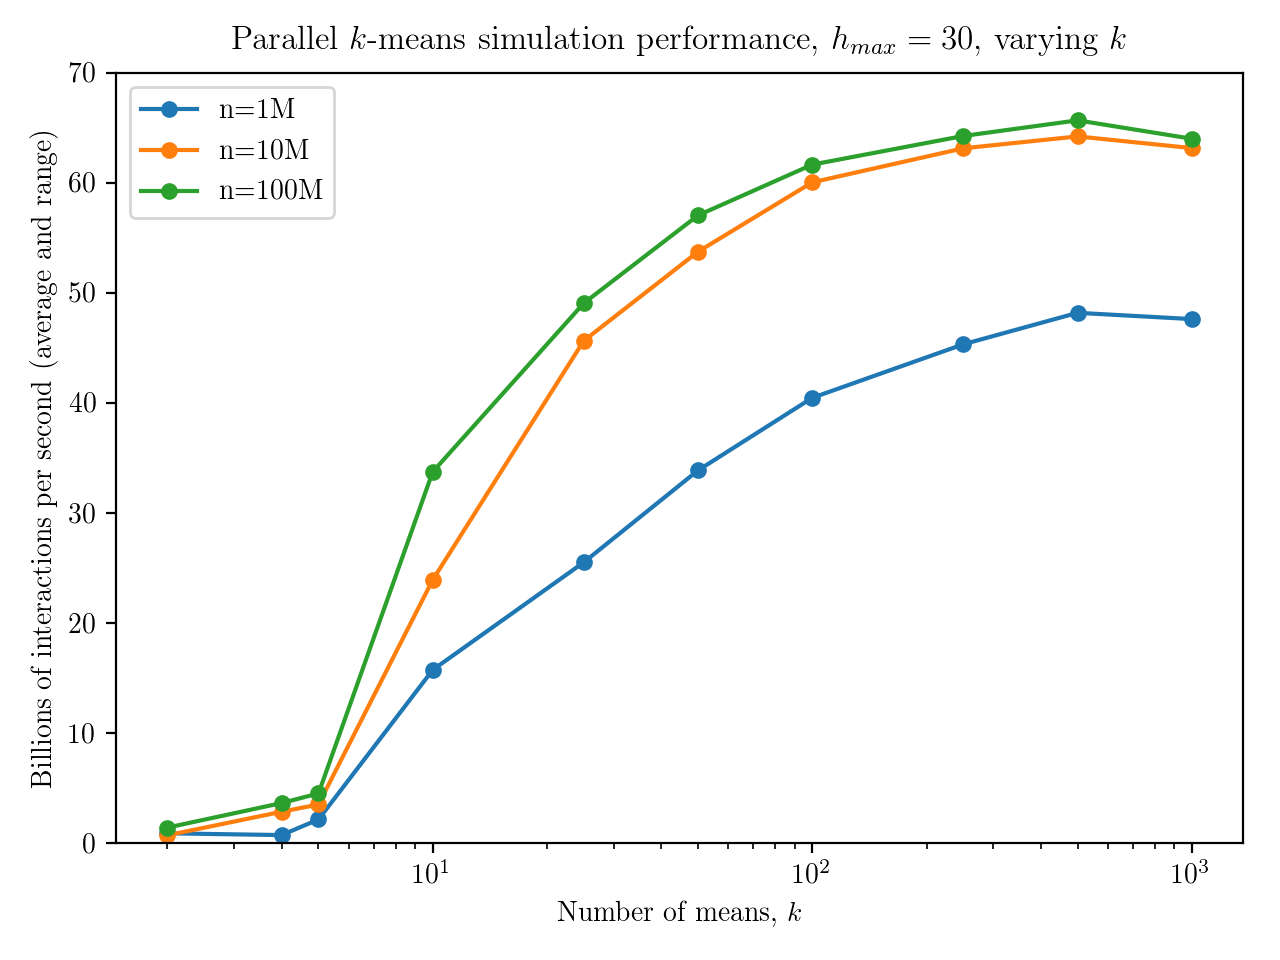
\includegraphics[width=5.2cm]{figures/perf_plot2_log.png}\quad
			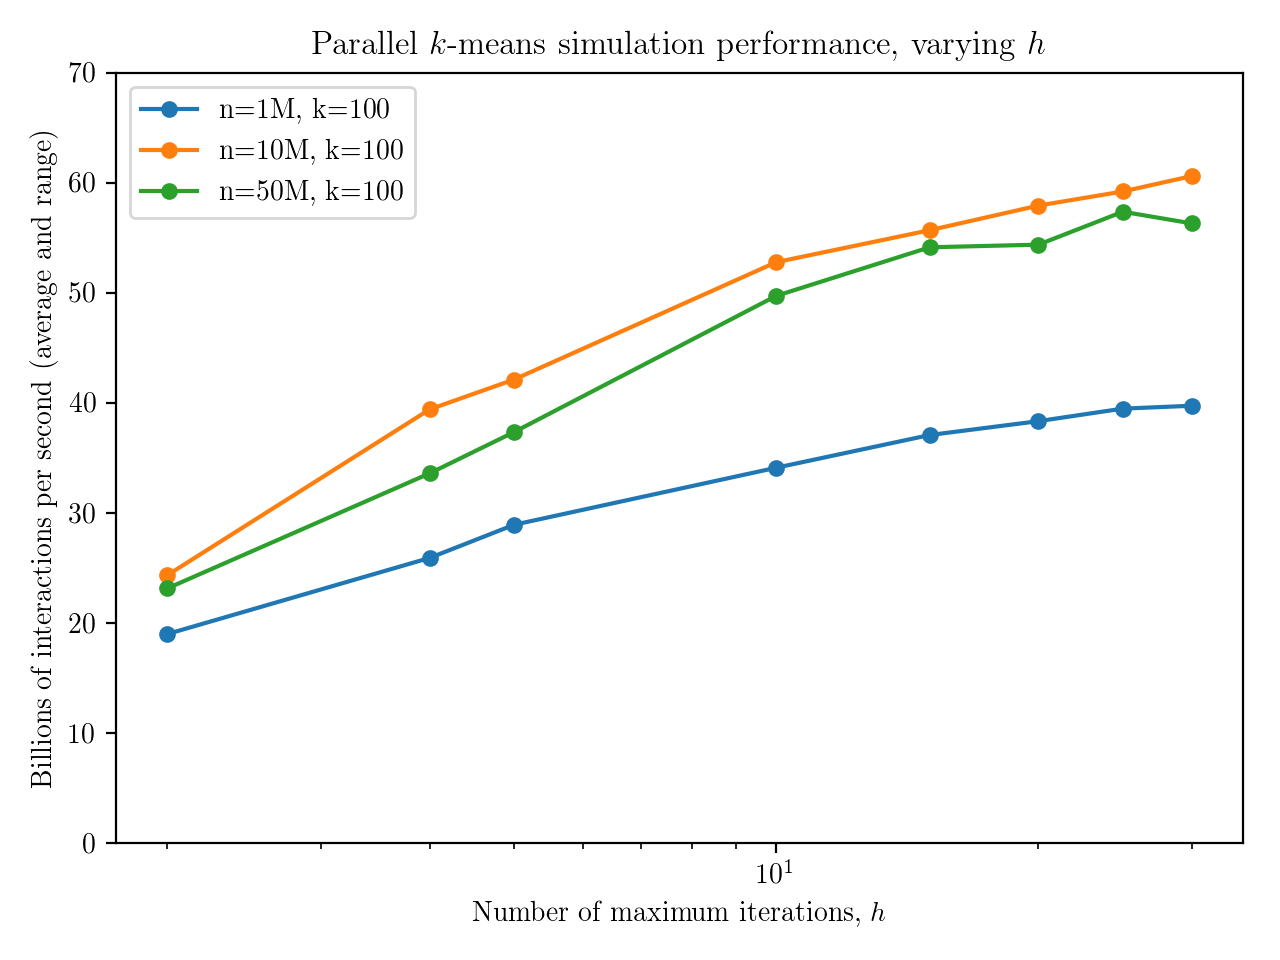
\includegraphics[width=5.2cm]{figures/perf_plot3_log.png}
		\end{center}
		\caption{Performance of the parallel algorithm (in log-scale) when compiled with \texttt{nvcc}. Left-Center-Right: Performance when varying $n$, $k$, and $h$, respectively.}
	\end{figure}

	\begin{figure}[H]
		\begin{center}
			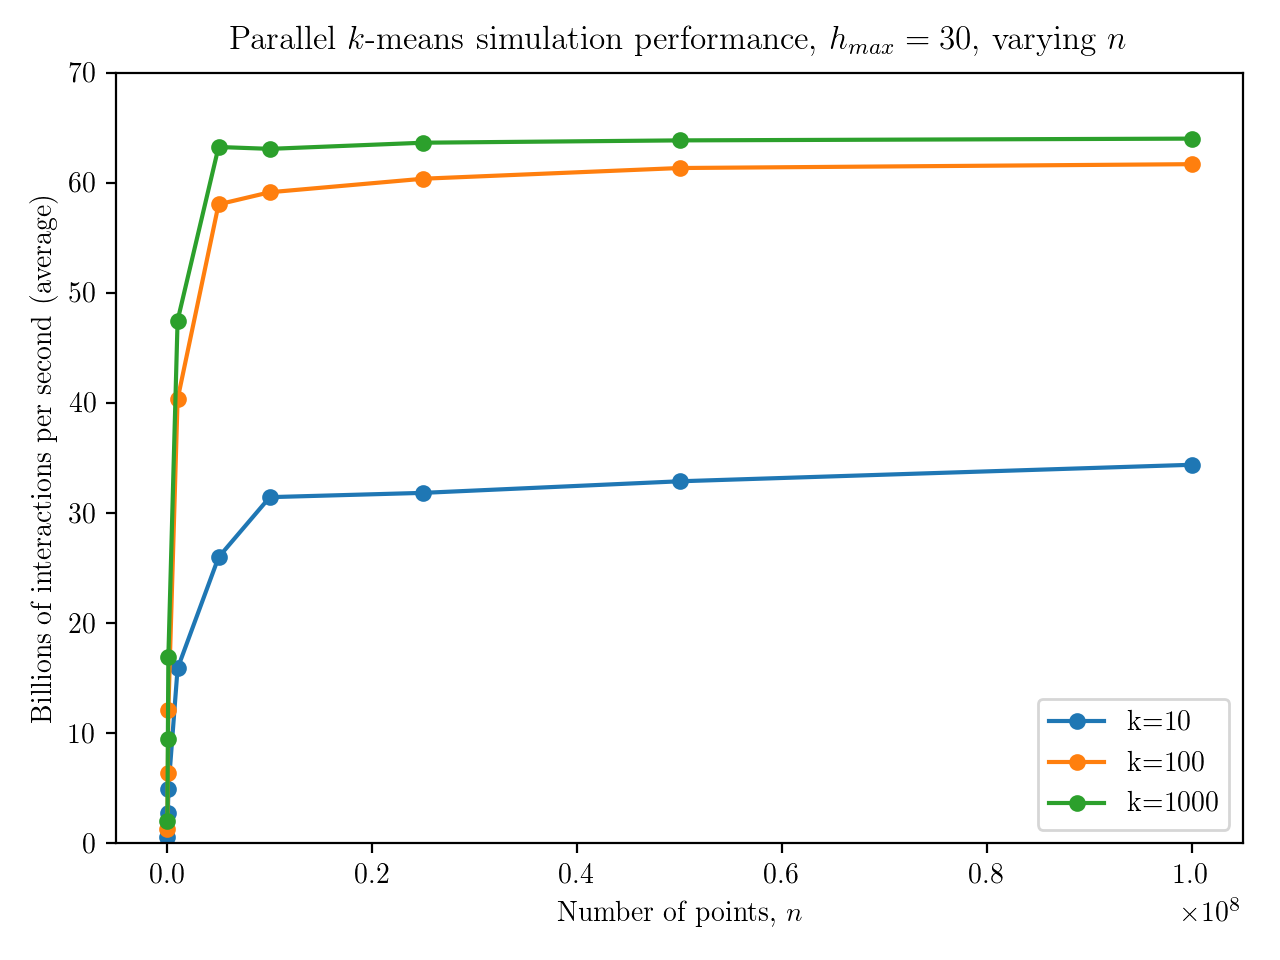
\includegraphics[width=5.2cm]{figures/perf_plot1_lin.png}\quad
			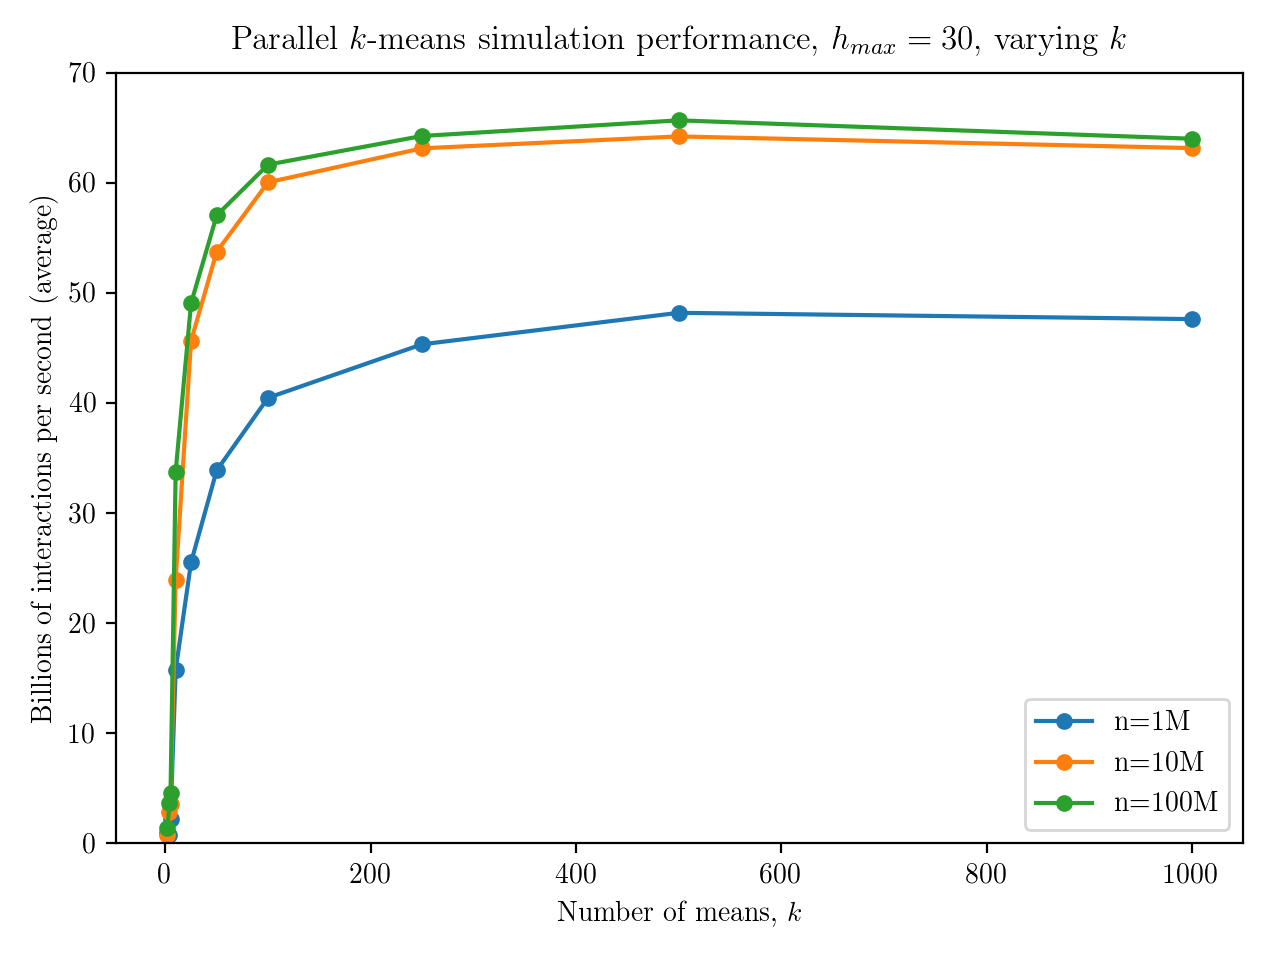
\includegraphics[width=5.2cm]{figures/perf_plot2_lin.png}\quad
			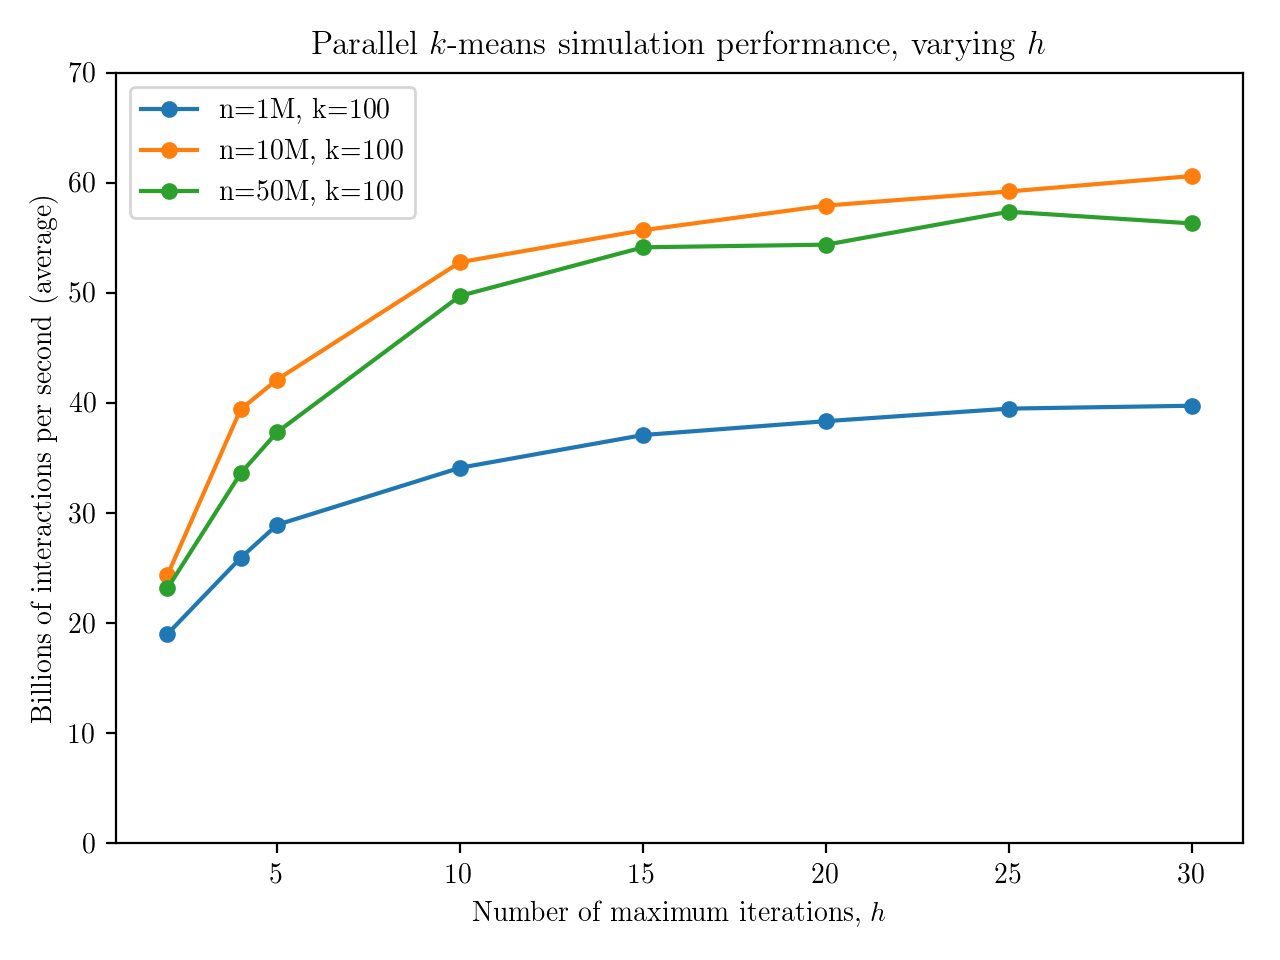
\includegraphics[width=5.2cm]{figures/perf_plot3_lin.png}
		\end{center}
		\caption{Performance of the parallel algorithm (in linear-scale) when compiled with \texttt{nvcc}. Left-Center-Right: Performance when varying $n$, $k$, and $h$, respectively.}
	\end{figure}
	
	\clearpage\subsection*{Sample Output}
	
	We wrote a short data generator in Python that draws points from 2D Gaussians on a radial tree.
	
	\lstset{
		language=Python,
		basicstyle=\scriptsize\ttfamily,
		keywordstyle=\color{blue}\ttfamily,
		stringstyle=\color{red}\ttfamily,
		commentstyle=\color{dkgreen}\ttfamily,
		tabsize=2,
		numbers=left,
		stepnumber=1,
		firstnumber=1,
		numberfirstline=true,
		numberstyle=\tiny
	}
	\begin{lstlisting}
import numpy as np
import sys

# 10 20 5 2 2000000 0.1 generates 100M points
num_branches1 = int(sys.argv[1])
dist_branches1 = float(sys.argv[2])
num_branches2 = int(sys.argv[3])
dist_branches2 = float(sys.argv[4])
cluster_size = int(sys.argv[5])
cluster_scale = float(sys.argv[6])

for i in range(num_branches1):
    for j in range(num_branches2):
        val = dist_branches1 * 1j ** (i * 4 / num_branches1) + \
              dist_branches2 * 1j ** (j * 4 / num_branches2)
        for _ in range(cluster_size):
            x = val.real + np.random.normal(scale=cluster_scale)
            y = val.imag + np.random.normal(scale=cluster_scale)
            print(x, y)
	\end{lstlisting}
	
	For example, the 1 million point data sets were generated with
	\[\texttt{python3 gen\_radial\_points.py 10 20 5 2 20000 0.1}\]
	yielding
	\begin{itemize}
		\item 10 ``large clusters'' 20 units away from the origin
		\item 5 ``small clusters'' in each large one, 5 units away from the centers of the large clusters.
		\item 20 thousand points per cluster, drawn from a 2D Gaussian distribution with standard deviation 0.1.
	\end{itemize}

	\begin{figure}[H]
		\begin{center}
			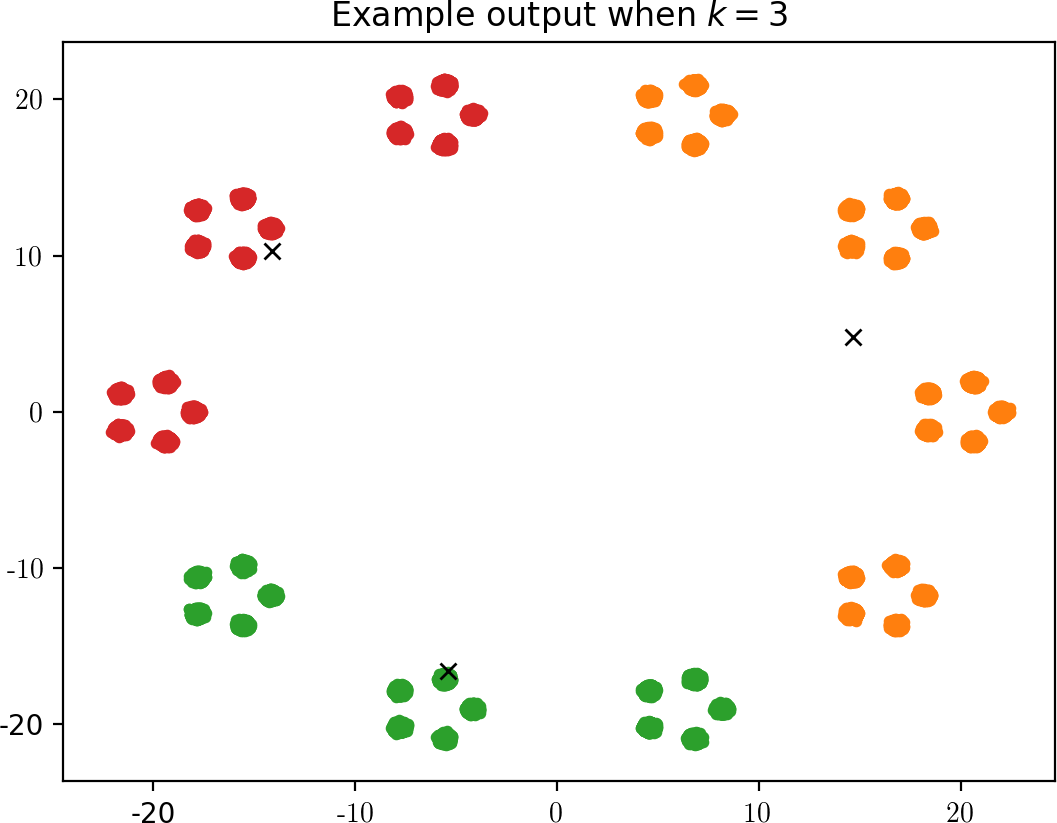
\includegraphics[width=5.2cm]{figures/Ex_k=3.png}\quad
			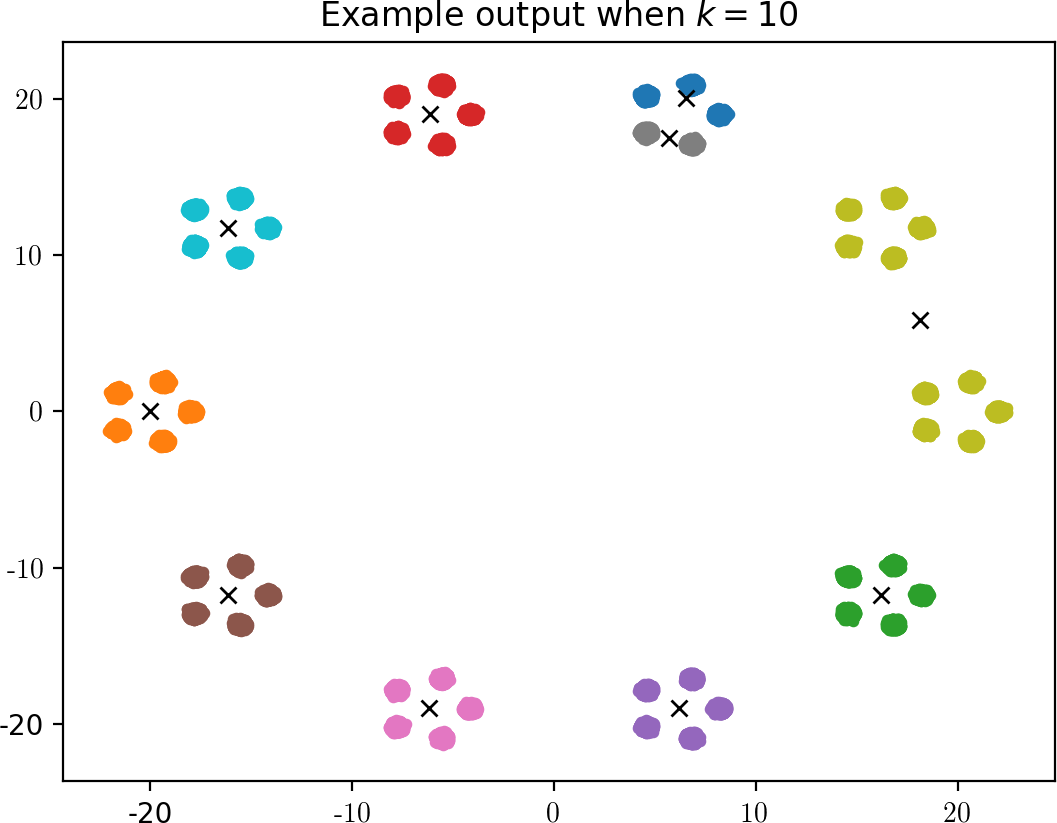
\includegraphics[width=5.2cm]{figures/Ex_k=10.png}\quad
			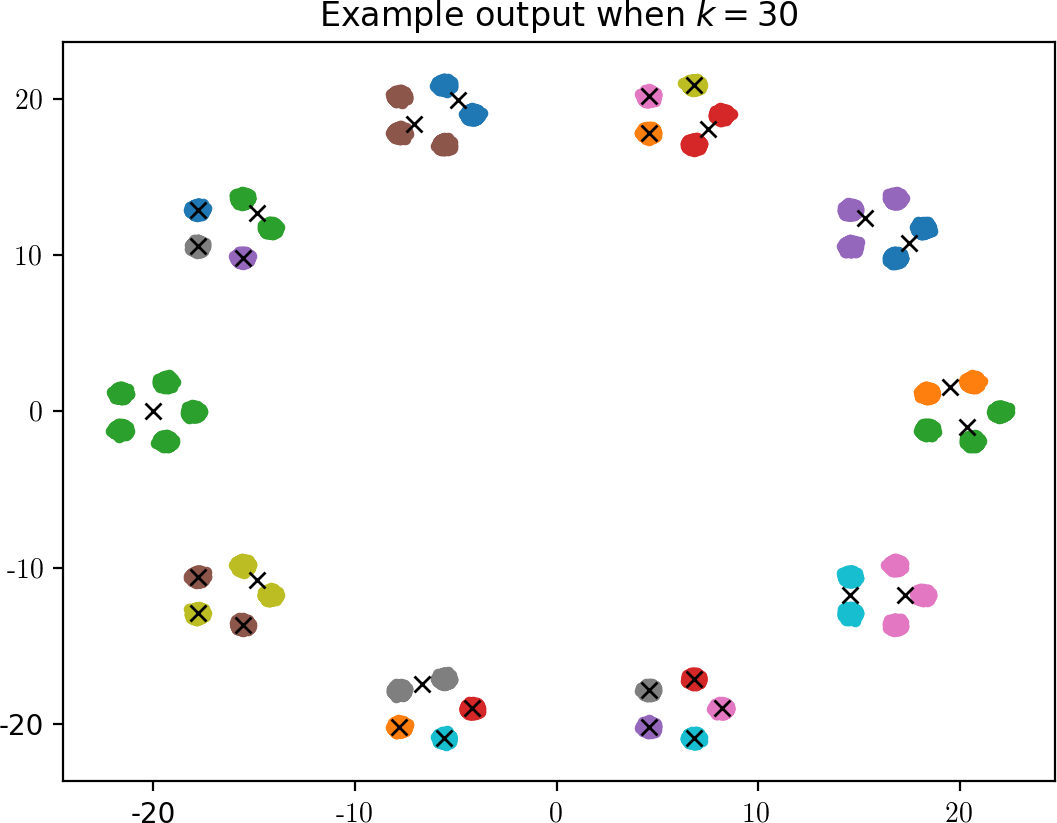
\includegraphics[width=5.2cm]{figures/Ex_k=30.png}
		\end{center}
		\caption{Example output from our parallel $k$-means algorithm. Left-Center-Right: Output with $k = 3, 10, 30$, respectively.}
	\end{figure}

	Strictly speaking, the CUDA/\CPP{} code simply prints a performance reading, followed by lines of the form
	\begin{alltt}
=====cluster 0 centered at 14.635420 4.755381 has size 400000=====
22.014330 -0.275197
21.905111 0.078775
21.974599 0.088757
<OMIT>
=====cluster 1 centered at -5.393562 -16.599389 has size 300000=====
-14.175596 -11.695731
-14.225406 -11.717935
-14.166853 -11.820264
<OMIT>
	\end{alltt}
	but this could be easily altered to have the results exported in other formats.
	
	\clearpage\subsection*{CUDA Code Listing}
	\lstset{
		language=C++,
		basicstyle=\scriptsize\ttfamily,
		keywordstyle=\color{blue}\ttfamily,
		stringstyle=\color{red}\ttfamily,
		commentstyle=\color{dkgreen}\ttfamily,
		tabsize=2,
		numbers=left,
		stepnumber=1,
		firstnumber=1,
		numberfirstline=true,
		numberstyle=\tiny,
		emph={
			cudaMallocManaged,
			__global__, __shared__, __device__, __host__,
			__syncthreads, __restrict__, __managed__
		},
		emphstyle=\color{red}\ttfamily,
	}
	\begin{lstlisting}
#include <assert.h>
#include <math.h>
#include <stdio.h>
#include <stdlib.h>
#include <string.h>
#include <time.h>

#define BLOCK_SIZE 512
#define MAX_POINTS 100000000 // 100M points
#define MAX_MEANS 1000
#define MAX_ITER 30

// CUDA prefers struct-of-arrays style here (for cache purposes)
typedef struct {
  double *x, *y;
  int *membership;
} points;

typedef struct {
  double *x, *y;
} centroids;

typedef struct {
  double *x_sum, *y_sum;
  int *size;
} temp_centroids;

// algorithm termination flag
__managed__ int assignment_changed = 1;

// reads n data points from input file
__host__ void read_data(int n, char *file_name, points P) {
  unsigned int i = 0;
  double x, y;
  FILE *file = fopen(file_name, "r");
  assert(file != NULL);

  while (!feof(file) && i < n) {
    if (fscanf(file, "%lf %lf", &x, &y) != 2)
      break;
    P.x[i] = x;
    P.y[i] = y;
    P.membership[i++] = -1;
  }
}

// selects k centers at random from n points
__host__ void init_centers(int n, int k, points P, centroids C) {
  srand(time(NULL));
  for (int i = 0; i < k; ++i) {
    // not actually uniform random sampling, but very close
    int rand_idx = rand() % n;
    C.x[i] = P.x[rand_idx];
    C.y[i] = P.y[rand_idx];
  }
}

// computes ||p-c||^2 for a point p and center c
__device__ inline double norm_2D_sqr(double x1, double y1,
                                     double x2, double y2) {
  // sqrt is monotonic, so we may omit it in the distance calculation
  // i.e. application of sqrt does not change the order of distances
  return (x1 - x2) * (x1 - x2) + (y1 - y2) * (y1 - y2);
}

// assign each point to the cluster given by the closest centroid
// NVIDIA suggests const and restrict here to improve compiler optimization
__global__ void
assign_clusters(int n, int k,
                const double *__restrict__ Px,
                const double *__restrict__ Py,
                int *__restrict__ Pmembership,
                double *__restrict__ Cx,
                double *__restrict__ Cy,
                double *__restrict__ Ox_sum,
                double *__restrict__ Oy_sum,
                int *__restrict__ Osize) {
  int index = blockIdx.x * blockDim.x + threadIdx.x;
  int tid = threadIdx.x;

  // thread-local values that will be reduced
  __shared__ double x_sum[BLOCK_SIZE];
  __shared__ double y_sum[BLOCK_SIZE];
  __shared__ int size[BLOCK_SIZE];

  int membership = -1;

  if (index < n) {
    double min_dist = INFINITY;
    for (int i = 0; i < k; ++i) {
      double current_dist = norm_2D_sqr(Px[index], Py[index], Cx[i], Cy[i]);
      if (current_dist < min_dist) {
        min_dist = current_dist;
        membership = i;
      }
    }

    // arbitrary concurrent write is valid since all
    // threads write the same value
    if (membership != Pmembership[index])
      assignment_changed = 1;
    Pmembership[index] = membership;
  }
  __syncthreads();

  // k reductions (one per centroid)
  for (int c = 0; c < k; ++c) {
    x_sum[tid] = (membership == c) ? Px[index] : 0;
    y_sum[tid] = (membership == c) ? Py[index] : 0;
    size[tid] = (membership == c) ? 1 : 0;
    __syncthreads();

    // reduce block's sums into one value (in thread 0)
    for (int offset = BLOCK_SIZE >> 1; offset > 0; offset >>= 1) {
      if (tid < offset) {
        x_sum[tid] += x_sum[tid + offset];
        y_sum[tid] += y_sum[tid + offset];
        size[tid] += size[tid + offset];
      }
      __syncthreads();
    }

    // save block's sums to output arrays
    if (tid == 0) {
      Ox_sum[blockIdx.x * k + c] = x_sum[tid];
      Oy_sum[blockIdx.x * k + c] = y_sum[tid];
      Osize[blockIdx.x * k + c] = size[tid];
    }
    __syncthreads();
  }
}

// reduce temporary cluster sizes and centroid x/y sums to smaller arrays
__global__ void
reduce_temp_clusters(int n, int k,
                     const double *__restrict__ Ix_sum,
                     const double *__restrict__ Iy_sum,
                     const int *__restrict__ Isize,
                     double *__restrict__ Ox_sum,
                     double *__restrict__ Oy_sum,
                     int *__restrict__ Osize) {
  int index = blockIdx.x * blockDim.x + threadIdx.x;
  int stride = blockDim.x * gridDim.x;
  int tid = threadIdx.x;

  // thread-local values that will be reduced
  __shared__ double x_sum[BLOCK_SIZE];
  __shared__ double y_sum[BLOCK_SIZE];
  __shared__ int size[BLOCK_SIZE];

  for (int c = 0; c < k; ++c) {
    x_sum[tid] = 0;
    y_sum[tid] = 0;
    size[tid] = 0;

    // if necessary, sum multiple items per thread
    for (int b = index; b < n; b += stride) {
      x_sum[tid] += Ix_sum[b * k + c];
      y_sum[tid] += Iy_sum[b * k + c];
      size[tid] += Isize[b * k + c];
    }
    __syncthreads();

    // reduce block's sums into one value (in thread 0)
    for (int offset = BLOCK_SIZE >> 1; offset > 0; offset >>= 1) {
      if (tid < offset) {
        x_sum[tid] += x_sum[tid + offset];
        y_sum[tid] += y_sum[tid + offset];
        size[tid] += size[tid + offset];
      }
      __syncthreads();
    }

    // save block's sums to output arrays
    if (tid == 0) {
      Ox_sum[blockIdx.x * k + c] = x_sum[tid];
      Oy_sum[blockIdx.x * k + c] = y_sum[tid];
      Osize[blockIdx.x * k + c] = size[tid];
    }
    __syncthreads();
  }
}

// update cluster centroid positions
__global__ void update_clusters(int n, int k,
                                double *__restrict__ Cx,
                                double *__restrict__ Cy,
                                const double *__restrict__ Ix_sum,
                                const double *__restrict__ Iy_sum,
                                const int *__restrict__ Isize) {
  int index = blockIdx.x * blockDim.x + threadIdx.x;

  if (index < k && Isize[index]) {
    Cx[index] = Ix_sum[index] / Isize[index];
    Cy[index] = Iy_sum[index] / Isize[index];
  }
}

/*
 *  prints results and performance where
 *    k = number of clusters (means)
 *    n = number of points (in 2D)
 *    h = number of iterations until convergence
 *    t = elapsed time (in seconds)
 *
 *    P contains the input points
 *    C contains the final cluster centroids
 *    T contains (in part) the final cluster sizes
 */
__host__ void print_results(int k, int n, int h, double t,
                            points P, centroids C, temp_centroids T) {
  printf("performed %d iterations in %.2f s, perf: %.2f billion\n", h, t,
         (double)k * n * h / t * 1e-9);

  double *xs = (double *)malloc(sizeof(double) * n);
  double *ys = (double *)malloc(sizeof(double) * n);
  int offsets[k + 1];

  offsets[0] = 0;
  for (int i = 0; i < k; ++i) {
    offsets[i + 1] = offsets[i] + T.size[i];
  }

  // pack permutation of input points into clusters in a single pass by using
  // prefix-sum on the cluster sizes as offsets into our output arrays
  for (int i = 0; i < n; ++i) {
    int m = P.membership[i];
    xs[offsets[m]] = P.x[i];
    ys[offsets[m]++] = P.y[i];
  }

  for (int c = 0; c < k; ++c) {
    printf("=====cluster %d centered at %lf %lf has size %d=====\n", c, C.x[c],
           C.y[c], T.size[c]);
    for (int i = offsets[c] - T.size[c]; i < offsets[c]; ++i) {
      printf("%lf %lf\n", xs[i], ys[i]);
    }
  }

  free(xs);
  free(ys);
}

int main(int argc, char **argv) {
  int k, n, h;
  char *file_name;
  points P;
  centroids C;
  temp_centroids T1;
  temp_centroids T2;
  cudaEvent_t start, stop;
  float time;

  // read in number of points and means
  assert(argc >= 4);
  n = atoi(argv[1]);
  k = atoi(argv[2]);
  file_name = argv[3];
  assert(n <= MAX_POINTS && k <= MAX_MEANS);

  int blockSize = BLOCK_SIZE;
  int numBlocks = (n + blockSize - 1) / blockSize;
  int reductionBlockSize = BLOCK_SIZE;
  int reductionNumBlocks =
      (numBlocks + reductionBlockSize - 1) / reductionBlockSize;

  // make sure that we can support the number of points with our two block
  // reductions. with BLOCK_SIZE = 512, this limit is ~250M points
  assert(reductionNumBlocks <= 1024);

  // malloc memory and set up GPU timers
  cudaMallocManaged(&P.x, sizeof(double) * n);
  cudaMallocManaged(&P.y, sizeof(double) * n);
  cudaMallocManaged(&P.membership, sizeof(int) * n);
  cudaMallocManaged(&C.x, sizeof(double) * k);
  cudaMallocManaged(&C.y, sizeof(double) * k);
  cudaMallocManaged(&T1.x_sum, sizeof(double) * numBlocks * k);
  cudaMallocManaged(&T1.y_sum, sizeof(double) * numBlocks * k);
  cudaMallocManaged(&T1.size, sizeof(int) * numBlocks * k);
  cudaMallocManaged(&T2.x_sum, sizeof(double) * reductionNumBlocks * k);
  cudaMallocManaged(&T2.y_sum, sizeof(double) * reductionNumBlocks * k);
  cudaMallocManaged(&T2.size, sizeof(int) * reductionNumBlocks * k);
  cudaEventCreate(&start);
  cudaEventCreate(&stop);

  read_data(n, file_name, P);
  init_centers(n, k, P, C);

  cudaEventRecord(start, 0);
  for (h = 0; assignment_changed && h < MAX_ITER; ++h) {
    // assign points to nearest clusters
    assignment_changed = 0;
    assign_clusters<<<numBlocks, blockSize>>>
      (n, k,
       P.x, P.y, P.membership,
       C.x, C.y,
       T1.x_sum, T1.y_sum, T1.size);
    cudaDeviceSynchronize();

    // two block reductions of cluster sizes and centroid x/y sums
    reduce_temp_clusters<<<reductionNumBlocks, reductionBlockSize>>>
      (numBlocks, k,
       T1.x_sum, T1.y_sum, T1.size,  // input values to reduce
       T2.x_sum, T2.y_sum, T2.size); // reduced output values
    cudaDeviceSynchronize();
    reduce_temp_clusters<<<1, reductionBlockSize>>>
      (reductionNumBlocks, k,
       T2.x_sum, T2.y_sum, T2.size,  // reduce values from T2
       T1.x_sum, T1.y_sum, T1.size); // back into T1
    cudaDeviceSynchronize();

    // update centroid positions
    update_clusters<<<1, k>>>
      (n, k,
       C.x, C.y,
       T1.x_sum, T1.y_sum, T1.size);
    cudaDeviceSynchronize();
  }

  cudaEventRecord(stop, 0);
  cudaEventSynchronize(stop);
  cudaEventElapsedTime(&time, start, stop);
  cudaEventDestroy(start);
  cudaEventDestroy(stop);

  print_results(k, n, h, time * 1e-3, P, C, T1);

  // CUDA automatically frees and resets device on program exit
}
	\end{lstlisting}
\end{document}
